\documentclass{article}
\usepackage{ctex}

\makeindex

\begin{document}

\section{Swirl Ratio}
The aspect ratio($A$) and swirl ratio($S$) are defined\cite{Natarajan-17}:
$$ A = \frac{H_0}{R_0} $$
$$ S = \frac{V_0}{2 A U_0} $$
where
\begin{description}
	\item[$R_0$: ] the radius of the updraft  in a tornado vortex chamber (Figure \ref{fig:TVC-diagram}).
	\item[$H_0$: ] the depth of inflow.
	\item[$U_0$: ] the radial velocity at $R_0$.
	\item[$V_0$: ] the axial velocity at $R_0$.
\end{description}

\begin{figure}
\centering
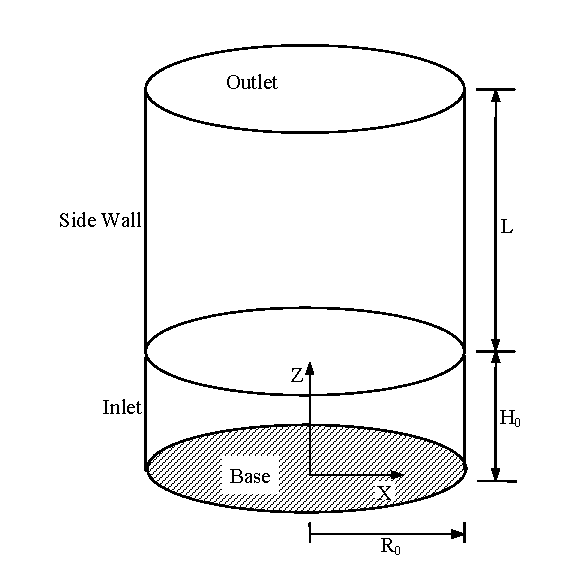
\includegraphics{_figure/TVC-diagram.pdf}
\caption[Schematic diagram of TVC]{Schematic diagram of the domain in the TVC model}
\label{fig:TVC-diagram}
\end{figure}


\bibliography{../_reference/tornado}
\bibliographystyle{plain}

\end{document}